% begin module limit-at-infinity-ex3
\begin{frame}
\begin{example}
\begin{columns}[c]
\column{.45\textwidth}
Evaluate $\lim\limits_{x\to \infty} \frac{3x^2-x-2}{5x^2+4x+1}$. %
\psset{xunit=0.55cm, yunit=0.55cm}
\begin{pspicture}(-5,-6.5)(5.1,2.1)
\psframe*[linecolor=white](-5,-6.5)(5.1,2.1)
\psaxes[ticks=none, labels=none]{<->}(0,0)(-5,-6.5)(5,2)
\fcLabelXOne

\uncover<21->{
\psline[linecolor=blue, linestyle=dashed](-5,0.6)(5, 0.6)
\rput[lb](1, 0.8) {\footnotesize$y=\frac{3}{5}=0.6$}
}

\uncover<23->{
%Function formula: (-2- (x)+3 ((x)^{2}))/(1+4 (x)+5 ((x)^{2}))
\psplot[linecolor=red, plotpoints=1000]{-4.95}{4.95}{x 2 exp 3 mul x -1 mul add -2 add x 2 exp 5 mul x 4 mul add 1 add div }
\rput[l](1, -2) {\footnotesize$y=\frac{3x^2-x-2}{5x^2+4x+1}$}
}
\end{pspicture}
%\ \only<handout:0| -20>{%
%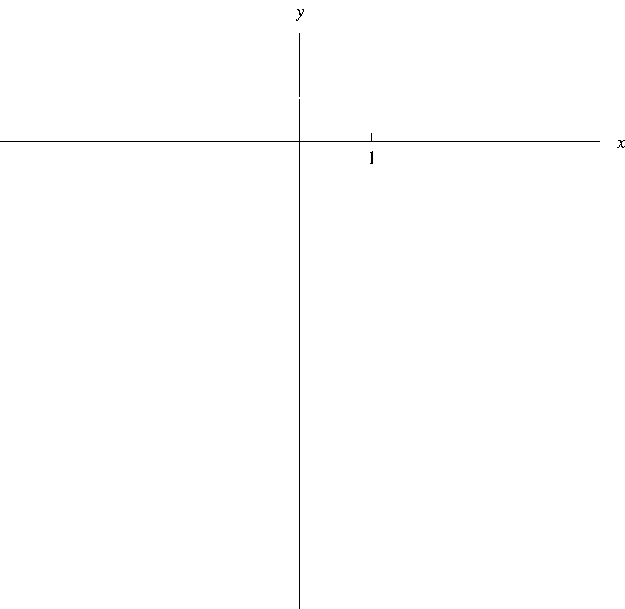
\includegraphics[width=5cm]{curve-sketching/pictures/04-04-ex3a.pdf}%
%}%
%\only<handout:0| 21-22>{%
%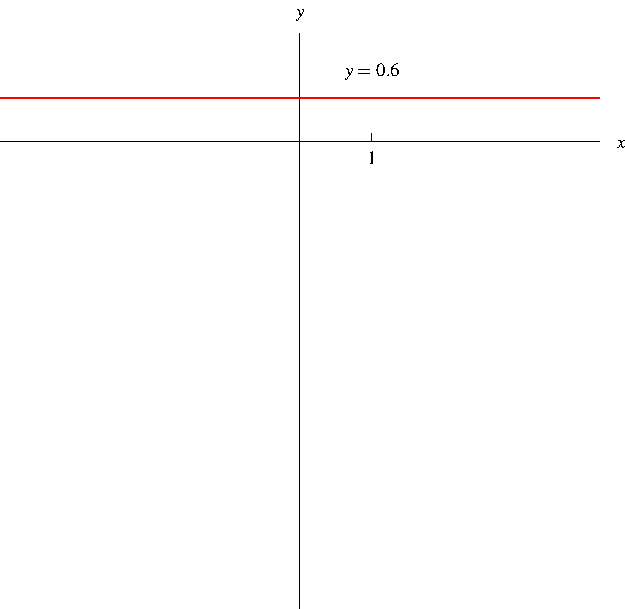
\includegraphics[width=5cm]{curve-sketching/pictures/04-04-ex3b.pdf}%
%}%
%\only<23->{%
%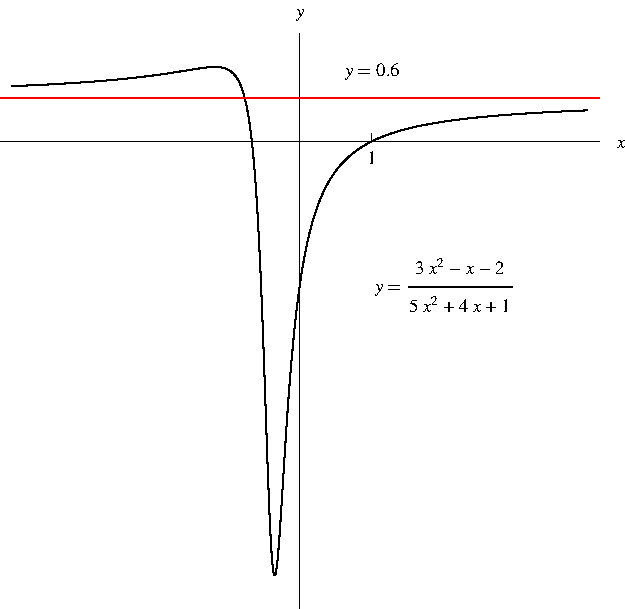
\includegraphics[width=5cm]{curve-sketching/pictures/04-04-ex3c.pdf}%
%}%
\uncover<22,23->{
A similar calculation shows that the limit as $x\to -\infty$ is also $\frac{3}{5}$.
}
\column{.55\textwidth}
\uncover<2->{\alertNoH{2,3}{Standard approach: divide top and bottom by the highest power of $x$ in the denominator.}}

$
\renewcommand{\arraystretch}{1.9}
\begin{array}{cl}
&\displaystyle
\lim\limits_{x\to \infty} \frac{\alertNoH{ 4-5}{\left(3x^2-x-2\right)}}{\left( \alertNoH{ 6-7}{ 5 \alertNoH{ 3}{x^2}+4x+1}\right) }\uncover<3->{\alertNoH{ 3}{\cdot \frac{\alertNoH{ 4-5}{\frac{1}{x^2}}}{\alertNoH{ 6-7}{\frac{1}{x^2}}}}}%
\\%
\uncover<4->{ = } &\displaystyle%
\uncover<4->{%
\alertNoH{9-20}{\lim\limits_{x\to \infty}} \frac{\fcAnswer{ 5}{ \alertNoH{9,10}{3} - \alertNoH{11,12}{\frac{1}{x}} - \alertNoH{13,14}{\frac{2}{x^2}}}}{\fcAnswer{ 7}{\alertNoH{15,16}{5}+\alertNoH{17,18}{\frac{4}{x}} + \alertNoH{19,20}{\frac{1}{x^2}}}}%
}%
\\%
 \uncover<8->{ = } &\displaystyle %
\uncover<8->{%
\frac{\displaystyle \alertNoH{ 9-10}{\lim_{x\to\infty}3} - \alertNoH{ 11-12}{\lim_{x\to\infty}\frac{1}{x}} - \alertNoH{ 13-14}{2 \lim_{x\to\infty}\frac{1}{x^2}}}{\displaystyle \alertNoH{ 15-16}{ \lim_{x\to\infty}5} + \alertNoH{ 17-18}{4 \lim_{ x\to \infty } \frac{1}{x}} + \alertNoH{ 19-20}{ \lim_{x \to \infty } \frac{1}{x^2}}}%
}%
\\%
 \uncover<9->{ = } &\displaystyle%
\uncover<9->{\frac{\fcAnswerUncover{9}{10}{3} - \fcAnswerUncover{9}{ 12}{0} - \fcAnswerUncover{9}{ 14}{0}}{\fcAnswerUncover{9}{ 16}{5} + \fcAnswerUncover{9}{ 18}{0} + \fcAnswerUncover{9}{ 20}{0}}}%
\uncover<21->{ = }%
\uncover<21->{\frac{3}{5}}%
\end{array}
$
\end{columns}
\end{example}
\end{frame}
% end module limit-at-infinity-ex3
